\documentclass{article}
\usepackage{../fasy-hw}

%% UPDATE these variables:
\renewcommand{\hwnum}{5}
\title{Discrete Structures, Homework \hwnum}
\author{Robert Marsh (JamesBean)}
\collab{n/a}
\date{due: 19 March 2021}

\begin{document}

\maketitle

This homework assignment should be
submitted as a single PDF file both to D2L and to Gradescope.

General homework expectations:
\begin{itemize}
    \item Homework should be typeset using LaTex.
    \item Answers should be in complete sentences and proofread.
    \item You will not plagiarize.
    \item List collaborators at the start of each question using the \texttt{collab} command.
    \item Put your answers where the \texttt{todo} command currently is (and
        remove the \texttt{todo}, but not the word \texttt{Answer}).
\end{itemize}


% ============================================
% ============================================
\collab{} \nextprob{Colors}
% ============================================
% ============================================

One thing that we need to consider as computer scientists is making our products
(software, technical papers) accessible to a wide range of people. When
designing GUIs or writing technical papers (e.g., journal papers or even
homework solutions), explain five things that you could do to make your
technical write-ups, website, or GUI products more accessible to people who
might be colour deficient or have Colour deficiency(or have a bad computer screen).


\paragraph{Answer}

\begin{enumerate}
    \item \textbf{Test it.} The overarching direction that helps create accessible  material is making sure that everything works well in complete greyscale, with no color at all. Test your content through a greyscale lens before sending it out.
    \item \textbf{Label Everything.} Color is commonly used as a labeling mechanism to identify different regions. In an environment with clear borders and a small number of elements, labeling each with a text description can be enough.
    \item \textbf{Use "good" colors.} When using color for emphasis (such as colored buttons in a GUI, or arbitrarily colored lines on graphs), use colors with high contrast that are visible to those with colorblindness. Black on white is the simplest, the extension being dark-on-light and light-on-dark pairs with contrast that is visible in greyscale. As there are different types of colorblindness/weakness, it's not possible to create ideal color schemes for all types at once.
    \item \textbf{Use patterns/textures.} Instead of just color, add high contrast textures/repeating patterns. Thanks to the four-color theorem, maps can be colored in entirely black and white with just hash marks ($0^{\circ}$vertical, $90^{\circ}$horizontal, diagonal $45^{\circ}$, diagonal $135^{\circ}$). With the addition of simple symbol patterns, there are a plethora of distinct patterns that can create visual distinction on maps, graphs, buttons and GUI areas.
    \item \textbf{Use different sizes and shapes and locations.} For websites and GUI products, color is often used to catch the eye and highlight specific buttons or visual areas. In a greyscale environment, varying size and shape is a good alternative. There's a lot of default rectangular shapes and 12pt text. Uncommon shapes (stars, circles, pentagons) in key locations (the middle and top of the screen) can stand out, highlighting important buttons/information, and larger text is more easily seen at a glance. The converse of this is commonly seen in spam emails - the link to unsubscribe is in small plain text at the bottom of the email, to avoid being seen.
\end{enumerate}



% ============================================
% ============================================
\collab{} \nextprob{The Complete Bipartite Graph $K_{n,n}$}
% ============================================
% ============================================

How many edges does the complete bipartite graph $K_{n,n}$ have?  Make your
conjecture, then prove that it is correct.

Bonus: Instead, prove the more general case:
what is the number of edges in $K_{n,m}$?

\paragraph{Answer}

The complete bipartite graph $K_{n,n}$ has $n^2$ edges.

\textbf{Proof (by mathematical induction):} Let $P(n)$ be the sentence
\begin{align}
    \nonumber \text{the complete bipartite graph $K_{n,n}$ has $n^2$ edges.} && \leftarrow P(n)
\end{align}

\emph{\textbf{Show that P(0) is true:}} \newline
$P(0)$ is true because a graph with no vertices has 0 edges.

\emph{\textbf{Show that P(1) is true:}} \newline
By definition of complete bipartite graph, $K_{1,1}$ is a simple graph with distinct vertices $v_1$ and $w_1$ and an edge from $v_1$ to $w_1$. Hence, $P(1)$ is true.

\emph{\textbf{Show that for all integers $k \geq 1$, if P(k) is true then P(k+1) is also true:}}
\newline \emph{[Suppose that P(k) is true for a particular but arbitrarily chosen integer $k \geq 1$. That is:]} \newline
Suppose that $k$ is any integer with $k \geq 1$ such that
\begin{align}
    \nonumber \text{the complete bipartite graph $K_{k,k}$ has $k^2$ edges.} && \leftarrow P(k), \text{\emph{the inductive hypothesis}}
\end{align}
\emph{[We must show that P(k+1) is true. That is:]} We must show that
\begin{align}
    \nonumber \text{the complete bipartite graph $K_{k+1,k+1}$ has $(k+1)^2$ edges.} && \leftarrow P(k+1)
\end{align}

By definition of complete bipartite graph, $K_{k+1,k+1}$ is a simple graph with distinct vertices $v_1, v_2,...,v_{k+1}$ and $w_1, w_2,...,w_{k+1}$ that satisfies the following properties: For all $a,c = 1,2,...,k+1$ and for all $b,d = 1,2,...,k+1,$
\begin{enumerate}
    \item There is an edge from each vertex $v_a$ to each vertex $w_b$.
    \item There is no edge from any vertex $v_a$ to any other vertex $v_c$.
    \item There is no edge from any vertex $v_b$ to any other vertex $v_d$.
\end{enumerate}
By property 1, each vertex $v_a$ has one edge to each vertex $w_b$. There are $k+1$ vertices in $w$, so we count $k+1$ edges for each vertex $v$. Because there are $k+1$ vertices in $v$, so we count $k+1$ edges $k+1$ times, which is equal to $(k+1)^2$.\newline
\emph{[This is what we needed to show.]}\newline
\emph{[Since we have proved the basis step and the inductive step, we conclude that the proposition is true.]}





% ============================================
% ============================================
\collab{} \nextprob{Four Colors Suffice}
% ============================================
% ============================================

Read Chapters $7$ and $8$ of \emph{Four Colors Suffice}.

\begin{enumerate}

    \item In the Four Colors Suffice book, we saw the definition of Euler's
        Formula for a finite decomposition of a Sphere or 2-plane into vertices,
        edges, and faces.  What is the other formula known as Euler's formula?

        \paragraph{Answer}

        Euler's "other" formula is $e^{ix} = \cos x + i \sin x$, where $e$ is the natural number (also known as Euler's number), $i$ is the imaginary number $\sqrt{-1}$, and $x$ is any real number. This is important because it defines a relationship between trigonometry and the complex exponential function.

        My source for this question is: \url{https://en.wikipedia.org/wiki/Euler%27s_formula}
        
    \item  Consider the following construction: Start with a solid cube.  Then, slice
        off a small region around each vertex (image you have a sharp knife, so you take
        off a tetrahedron at each corner).  How many vertices, edges, and faces are on
        the surface of this object before and after this operation? What polyhedron is this?

        \paragraph{Answer} 
        Before: 8 vertices, 6 faces, 12 edges. After: 24 vertices, 14 faces, 36 edges.
        This is a truncated cube.



    \item Draw a projection of the octahedron onto the plane such that edges only
        intersect at vertices.  Can every polyhedron be drawn in such a way?

        \paragraph{Answer}
        Every convex polyhedron can be drawn in such a way, because they can be placed inside a sphere and have every point successfully projected onto the sphere.
        \begin{figure}[b!]
            \centering
            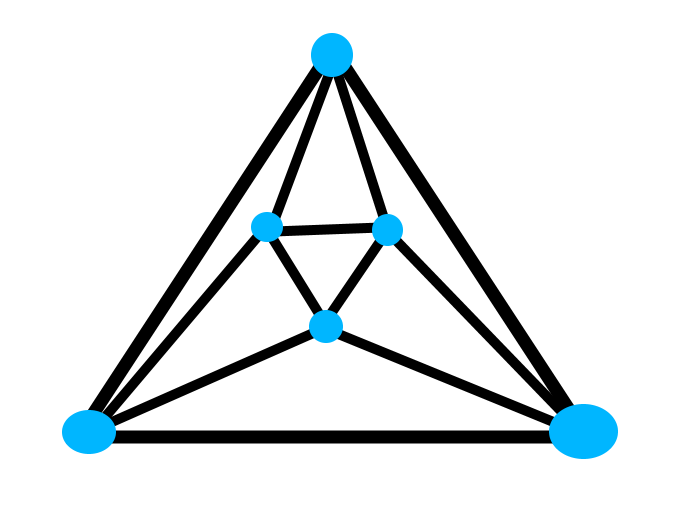
\includegraphics[width=150px]{octahedron.png}
            \caption{Projection of The Octahedron}
            \label{fig:Octahedron}
          \end{figure}


\end{enumerate}

% ============================================
% ============================================
\collab{}
\nextprob{Fran Allen}
% ============================================
% ============================================

Write a short (1-2 paragraph) biography of Fran Allen.
\textbf{In your own words}, describe who they are and why they are important in
the history of computer science.

If you use external resources, please provide
proper citations. If you do not use external sources, please write ``I did not
use any sources to write this biography'' as the last sentence of the
biography.

\paragraph{Answer}

Frances 'Fran' Allen was a 20-21st century computer scientist from the United States. Born in 1932, she grew up in a small town in New York before obtaining her bachelor's degree in mathematics in 1954. A few years later she return for her Master of Science in Mathematics at the University of Michigan, graduating in 1957. Returning to New York, she started a job at IBM teaching incoming employees Fortran, and stayed with them for the next 45 years. Eventually she moved into the realm of compiler optimization, working on code breaking projects for the NSA, and published several papers on compiler optimization. She had a short stint as a professor at New York University and Stanford University in the 70's, before returning to IBM to work on parallel computing. She received several awards for her work, most notable the A. M. Turing Award in 2006 for her work and publishing on compiler optimization and setting the standard for managing program dependence in parallel compiling. She passed away in 2020, on her birthday.

Frances' work, like many others, is important in the history of computer science because of the doors that it opens for the future. She developed new standards for analysis of compilers, and analysis of optimizing data flow in serial and parallel compilers. More efficient compilers allow for creating of more complex and more abstracted (higher level) programming languages. This allows experienced computer scientists to work on more complex problems by abstracting away the lower level details, and allows creation of simpler programming languages. Simpler programming languages lowers the barrier of entry for inexperienced computer scientists to learn about and enter the field. It also increases the ease of interdisciplinary collaboration between existing programmers and experts in other fields (by making it easy for non-programmers to learn about the field and communicate with computer scientists).

My source for this question is:
\begin{enumerate}
    \item \url{https://en.wikipedia.org/wiki/Frances_Allen}
\end{enumerate}


% %% ... the bibliography
% \newpage
% \bibliographystyle{acm}
% \bibliography{biblio}

\end{document}

